% 1989 年上海卷第七题：题设几何关系及坐标示意；两图均不表示精确比例
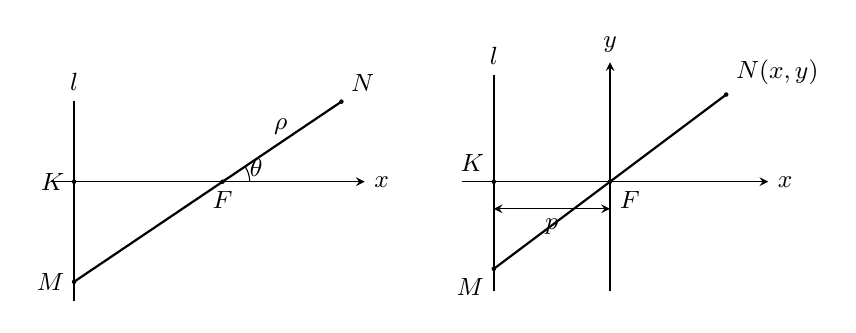
\begin{tikzpicture}[scale=0.82,>=stealth,font=\small]
  % Polar construction
  \begin{scope}
    \coordinate (K) at (0,0);
    \coordinate (F) at (2.3,0);
    \coordinate (M) at (0,-1.55);
    \coordinate (N) at (4.14,1.24);
    \draw[thick] (0,-1.85)--(0,1.25) node[above] {$l$};
    \draw[->] (-0.35,0)--(4.5,0) node[right] {$x$};
    \draw[thick] (M)--(N);
    \fill (K) circle (1pt) node[left] {$K$};
    \fill (F) circle (1pt) node[below] {$F$};
    \fill (M) circle (1pt) node[left] {$M$};
    \fill (N) circle (1pt) node[above right] {$N$};
    \draw (2.72,0) arc[start angle=0,end angle=33.98,radius=0.42];
    \node at (2.82,0.22) {$\theta$};
    \node at (3.2,0.85) {$\rho$};
  \end{scope}
  % Cartesian construction
  \begin{scope}[xshift=8.3cm]
    \coordinate (F) at (0,0);
    \coordinate (K) at (-1.8,0);
    \coordinate (M) at (-1.8,-1.35);
    \coordinate (N) at (1.8,1.35);
    \draw[thick] (-1.8,-1.7)--(-1.8,1.65) node[above] {$l$};
    \draw[->] (-2.3,0)--(2.45,0) node[right] {$x$};
    \draw[->] (0,-1.7)--(0,1.85) node[above] {$y$};
    \draw[thick] (M)--(N);
    \draw[<->] (-1.8,-0.42)--(0,-0.42) node[midway,below] {$p$};
    \fill (K) circle (1pt) node[above left] {$K$};
    \fill (F) circle (1pt) node[below right] {$F$};
    \fill (M) circle (1pt) node[below left] {$M$};
    \fill (N) circle (1pt) node[above right] {$N(x,y)$};
  \end{scope}
\end{tikzpicture}
